\documentclass[12pt]{article}

\usepackage[a4paper, margin=2cm]{geometry}

\setlength{\marginparwidth}{0pt}

\usepackage[utf8]{inputenc}
\usepackage[english]{babel}
\usepackage{datetime}

\usepackage{setspace}
\setstretch{1.2}

\usepackage{fancyhdr}
\setlength{\headheight}{15pt}
\usepackage{lastpage}
\renewcommand\headrulewidth{0pt}
\renewcommand\footrulewidth{0.3pt}
\fancyhead{}
\fancyfoot[C]{\thepage ~/ \pageref{LastPage}}
\pagestyle{fancy}

\usepackage{amsmath, amssymb}
\usepackage{graphicx}
\usepackage{color}


\begin{document}

\title{Part 2 -- Terrain Rendering}
\author{Éloi \textsc{Alain} \and Enguerrand \textsc{Granoux} \and Josselin \textsc{Held}}
\newdate{date}{04}{05}{2017}
\date{\displaydate{date}}

\maketitle

\tableofcontents

\section{Introduction}



\section{Mandatory parts}

\subsection{Realistic texture}

\subsubsection{Mapping with interpolation, randomness and steep slopes}

{\it Main contributor: Enguerrand.}

At first, we use the height to set up textures (sand, grass, rock and snow). Then we use some mix to have more realistic texture. The coefficient of the mix depends on the inclination and on the height. We also add a time dependence to represent the seasons and make the snow disappear.

\subsubsection{Improving steep slopes and realistic beaches}

{\it Main contributor: Éloi.}

The condition on the inclination -- computed with \texttt{dFdx} and \texttt{dFdy} -- only introduced pixel sparkling at the borders. In order to reduce the effect, I changed the condition structure to focus on water vs grass vs snow. The sand and rocks are then mixed with the grass -- using custom interpolation curves -- depending on the inclination of the slope (and altitude for the sand). Beaches do not occur on steep slopes.
  

\subsection{Skybox}

{\it Main contributor: Éloi.}

At first, I tried to map the cube pattern (presented during the class) onto the box using \texttt{glDrawElements}. Unfortunately, some vertices ought to be mapped to several points on the pattern.

Eventually, following the instructions on \texttt{learnopengl.com}, the result was better. The use of \texttt{\textsc{GL\_TEXTURE\_CUBE\_MAP}} was determining.


\section{Optional parts}

\subsection{Infinite terrain}

\subsubsection{Terrain movement}

{\it Main contributor: Éloi.}

When pressing the \textsc{w, a, s} and \textsc{d} keys the terrain moves continuously with time in the view direction. The principle used is to compute the noise at a position \texttt{(x, y)} on the grid that changes with time. This offset is now computed in \texttt{main.cpp} where key actions are listened to. Note that the projection of the view direction onto the vertical axis is set to zero so the camera remains high and centered.


\subsubsection{FPS camera}

{\it Main contributor: Éloi.}

The user may dynamically (while pressing aforementioned movement keys) change the view direction with the mouse. The trackball mechanism has been changed completely. The zoom feature now moves the camera in the view direction (this time, the camera position in the world changes, so it is literally possible to go anywhere in the world: under the terrain, outside the skybox).


\subsection{Water reflection}

{\it Main contributor: Josselin.}

We are implementing water reflection. We used the same concept as in the Homework 4, namely reflecting the camera under the water. We then draw a second time the now reflected terrain in a framebuffer, which is sent to a \texttt{water.h} class, which draw a second plan at height zero representing the water with the reflection.

\section{Fraction of the Workload}


\begin{enumerate}
\item Éloi Alain: 40\%
\item Enguerrand Granoux: 30\%
\item Josselin Held: 30\%
\end{enumerate}

\section{Screenshot}

\begin{center}
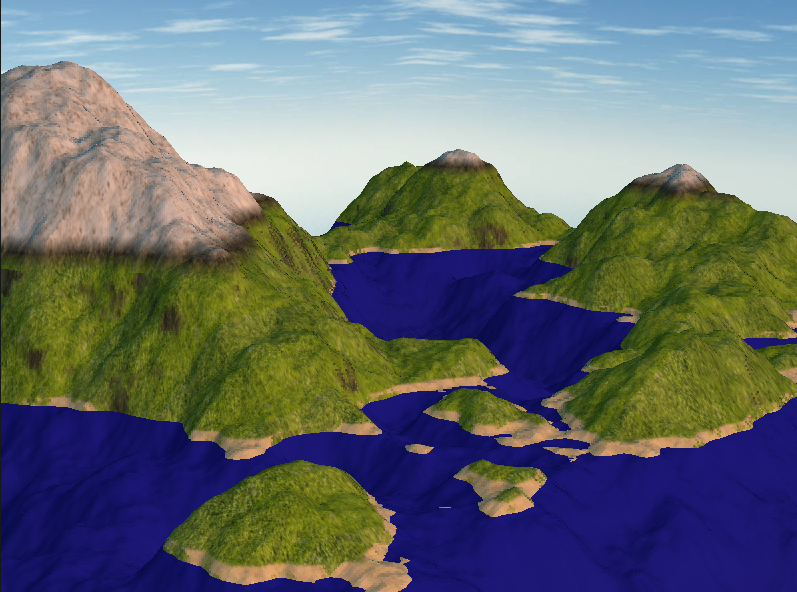
\includegraphics[width=15cm]{view.png}
\end{center}

\textcolor{red}{Waiting for water reflection}



% \begin{center}
% \includegraphics[width=15cm]{screeMontain.png}
% \end{center}


\end{document}

%  LocalWords:  Éloi Alain Enguerrand Granoux Josselin Perlin shader
%  LocalWords:  vec Framebuffer heightmap dFdx dFdy Rendering Held GL
%  LocalWords:  Mandatory Skybox glDrawElements learnopengl cpp
%  LocalWords:  skybox
